\documentclass[letterpaper,11pt,openany,oneside]{book}
% package includes
\usepackage{titlepic}
\usepackage{graphicx}
\usepackage{hyperref}
\usepackage{longtable}
\usepackage{ragged2e}
\usepackage{microtype}
\usepackage[table]{xcolor}
\usepackage[labelformat=empty]{caption}
% define the title
\author{CW2 Peter Goodspeed-Niklaus}
\title{HH-60 DA 2408-17 Photo Guide}
\titlepic{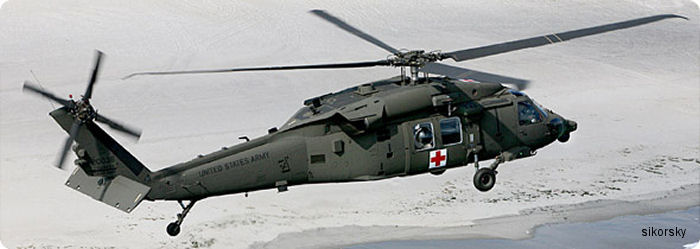
\includegraphics[width=\textwidth]{Images/hh-60m.jpg}}
% document options
\pagestyle{headings}
\newcolumntype{P}[1]{>{\RaggedRight\hspace{0pt}}p{#1}}

%%%%%%%%%%%%%%%%%%%%%%%%%%%%
% Document Starts Here     %
%%%%%%%%%%%%%%%%%%%%%%%%%%%%
\begin{document}
\frontmatter
% generates the title
\setcounter{page}{0}
\maketitle
\clearpage
\chapter*{About This Document}
Indices are identical but for ordering. First index is ordered per the part number on a reference DA~2408-17. Second index is ordered alphabetically by nomenclature.

For further information, reference TM 1-1520-237-23-9, Appendix~C: Aircraft Master Inventory Guide.

This document was generated in \LaTeXe. Source files may be found at \url{https://github.com/coriolinus/HH60-17photobook}. Fork the project for changes; pull requests will not be accepted. Tools used authoring this document include \href{http://texstudio.sourceforge.net/}{TeXstudio}\footnote{\url{http://texstudio.sourceforge.net/}}, \href{http://miktex.org/}{MiKTeX}\footnote{\url{http://miktex.org/}}, and \href{http://johnmacfarlane.net/pandoc/}{Pandoc}\footnote{\url{http://johnmacfarlane.net/pandoc/}}.

Document license: \href{https://creativecommons.org/}{Creative Commons} \href{https://creativecommons.org/licenses/by-sa/4.0/}{Attribution-ShareAlike 4.0 International}
\footnote{\url{https://creativecommons.org/licenses/by-sa/4.0/}}

\begin{center}
	\href{https://creativecommons.org/licenses/by-sa/4.0/}{
\includegraphics{Images/cc-by-sa.png}}
\end{center}

\mainmatter
\chapter{Index, DA~2408-17 Ordering}
\section{Section I: Cockpit}
\input{section1a.tex}
\clearpage
\section{Section II: Cabin}
\input{section2a.tex}
\clearpage
\section{Section III: Transition Section}
\input{section3a.tex}
\clearpage
\section{Section IV: Tail Cone}
\input{section4a.tex}
\clearpage
\section{Section V: Tail Rotor Pylon}
\input{section5a.tex}
\clearpage
\chapter{Index, Alphabetical by Nomenclature}
\section{Section I: Cockpit}
\input{section1b.tex}
\clearpage
\section{Section II: Cabin}
\input{section2b.tex}
\clearpage
\section{Section III: Transition Section}
\input{section3b.tex}
\clearpage
\section{Section IV: Tail Cone}
\input{section4b.tex}
\clearpage
\section{Section V: Tail Rotor Pylon}
\input{section5b.tex}
\clearpage
\chapter{Figures}
\begin{figure}[htp]
	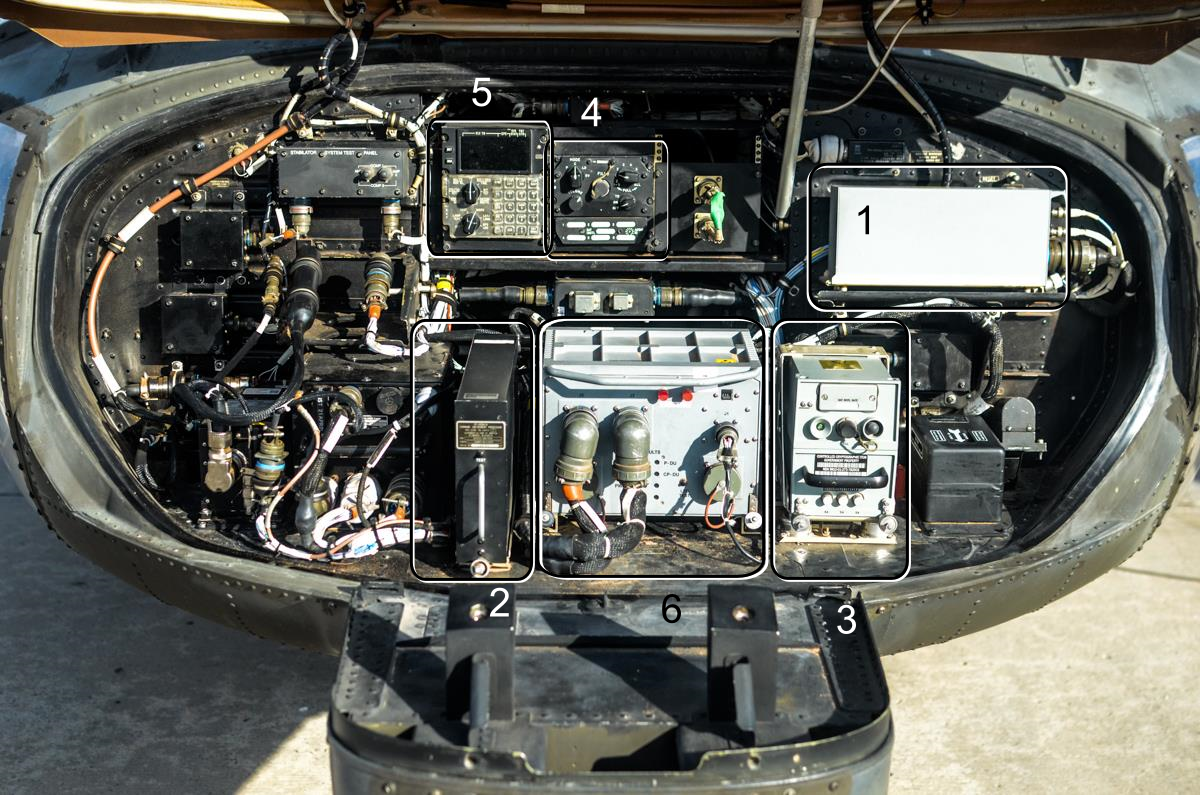
\includegraphics[width=\textwidth]{Images/avionics-bay.jpg}
	\caption{Avionics Bay} \label{avionics}
\end{figure}
\end{document}

